\chapter{Music Consumption Survey}\label{chap:survey}


\section{Background and objectives}
In order to better rationalize the topic of the thesis and show that a music streaming platform centered around social
interactions could be relevant as a service, a brief survey was conducted. It examines the
individual content‐consumption preferences, listening and discovery habits, platform usage patterns, and
social behaviours.


\section{Methods}
The platform chosen for the questionnaire was `Google Forms`\cite{googleforms}, as it provides a simple interface for
survey creation, allows for easy sharing of the form, and supports exporting the results to a spreadsheet.

The questionnaire itself consists of 15 questions.
Most of them are multi-choice and closed-ended with some having a possibility for a custom answer.
Custom answers are grouped under the "other" answer in the provided figures. Ungrouped answers could be found in the
original survey.

As for the respondents - 119 people had participated, with most being from Russian-speaking countries;
the majority was in the 18 to 30 age group, with the exact distribution shown in Figure~\ref{fig:age}.

The form can be accessed at: \url{https://docs.google.com/forms/d/1vhhAu_SfuHV4xy6JoDaRsM5uCElYn_csTmN8u4ZlpHc}

\begin{figure}[htbp]
    \centering
    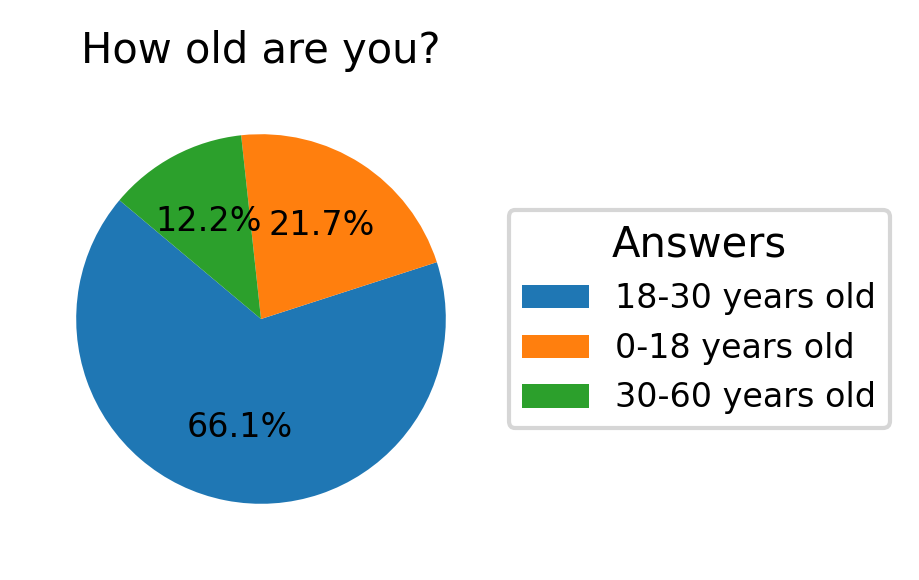
\includegraphics[width=0.8\textwidth, keepaspectratio]{charts/age.png}
    \caption{Age distribution of respondents}
    \label{fig:age}
\end{figure}


\section{Results}

\subsection{Engagement}
Firstly, it was necessary to determine the actual frequency of engagement with audio content -- if the numbers were low,
it would indicate that a dedicated platform with advanced features might not be relevant for most users.
However, over 50\% of respondents reported listening to more than 500 songs per month (Figure~\ref{fig:song_amount}),
and nearly 80\% stated that they listen to music daily (Figure~\ref{fig:listen_reg}).
This clearly shows that music is essential to many people, and the following logical step would be to discover
how the audio content is mostly accessed.

\begin{figure}[htbp]
    \centering
    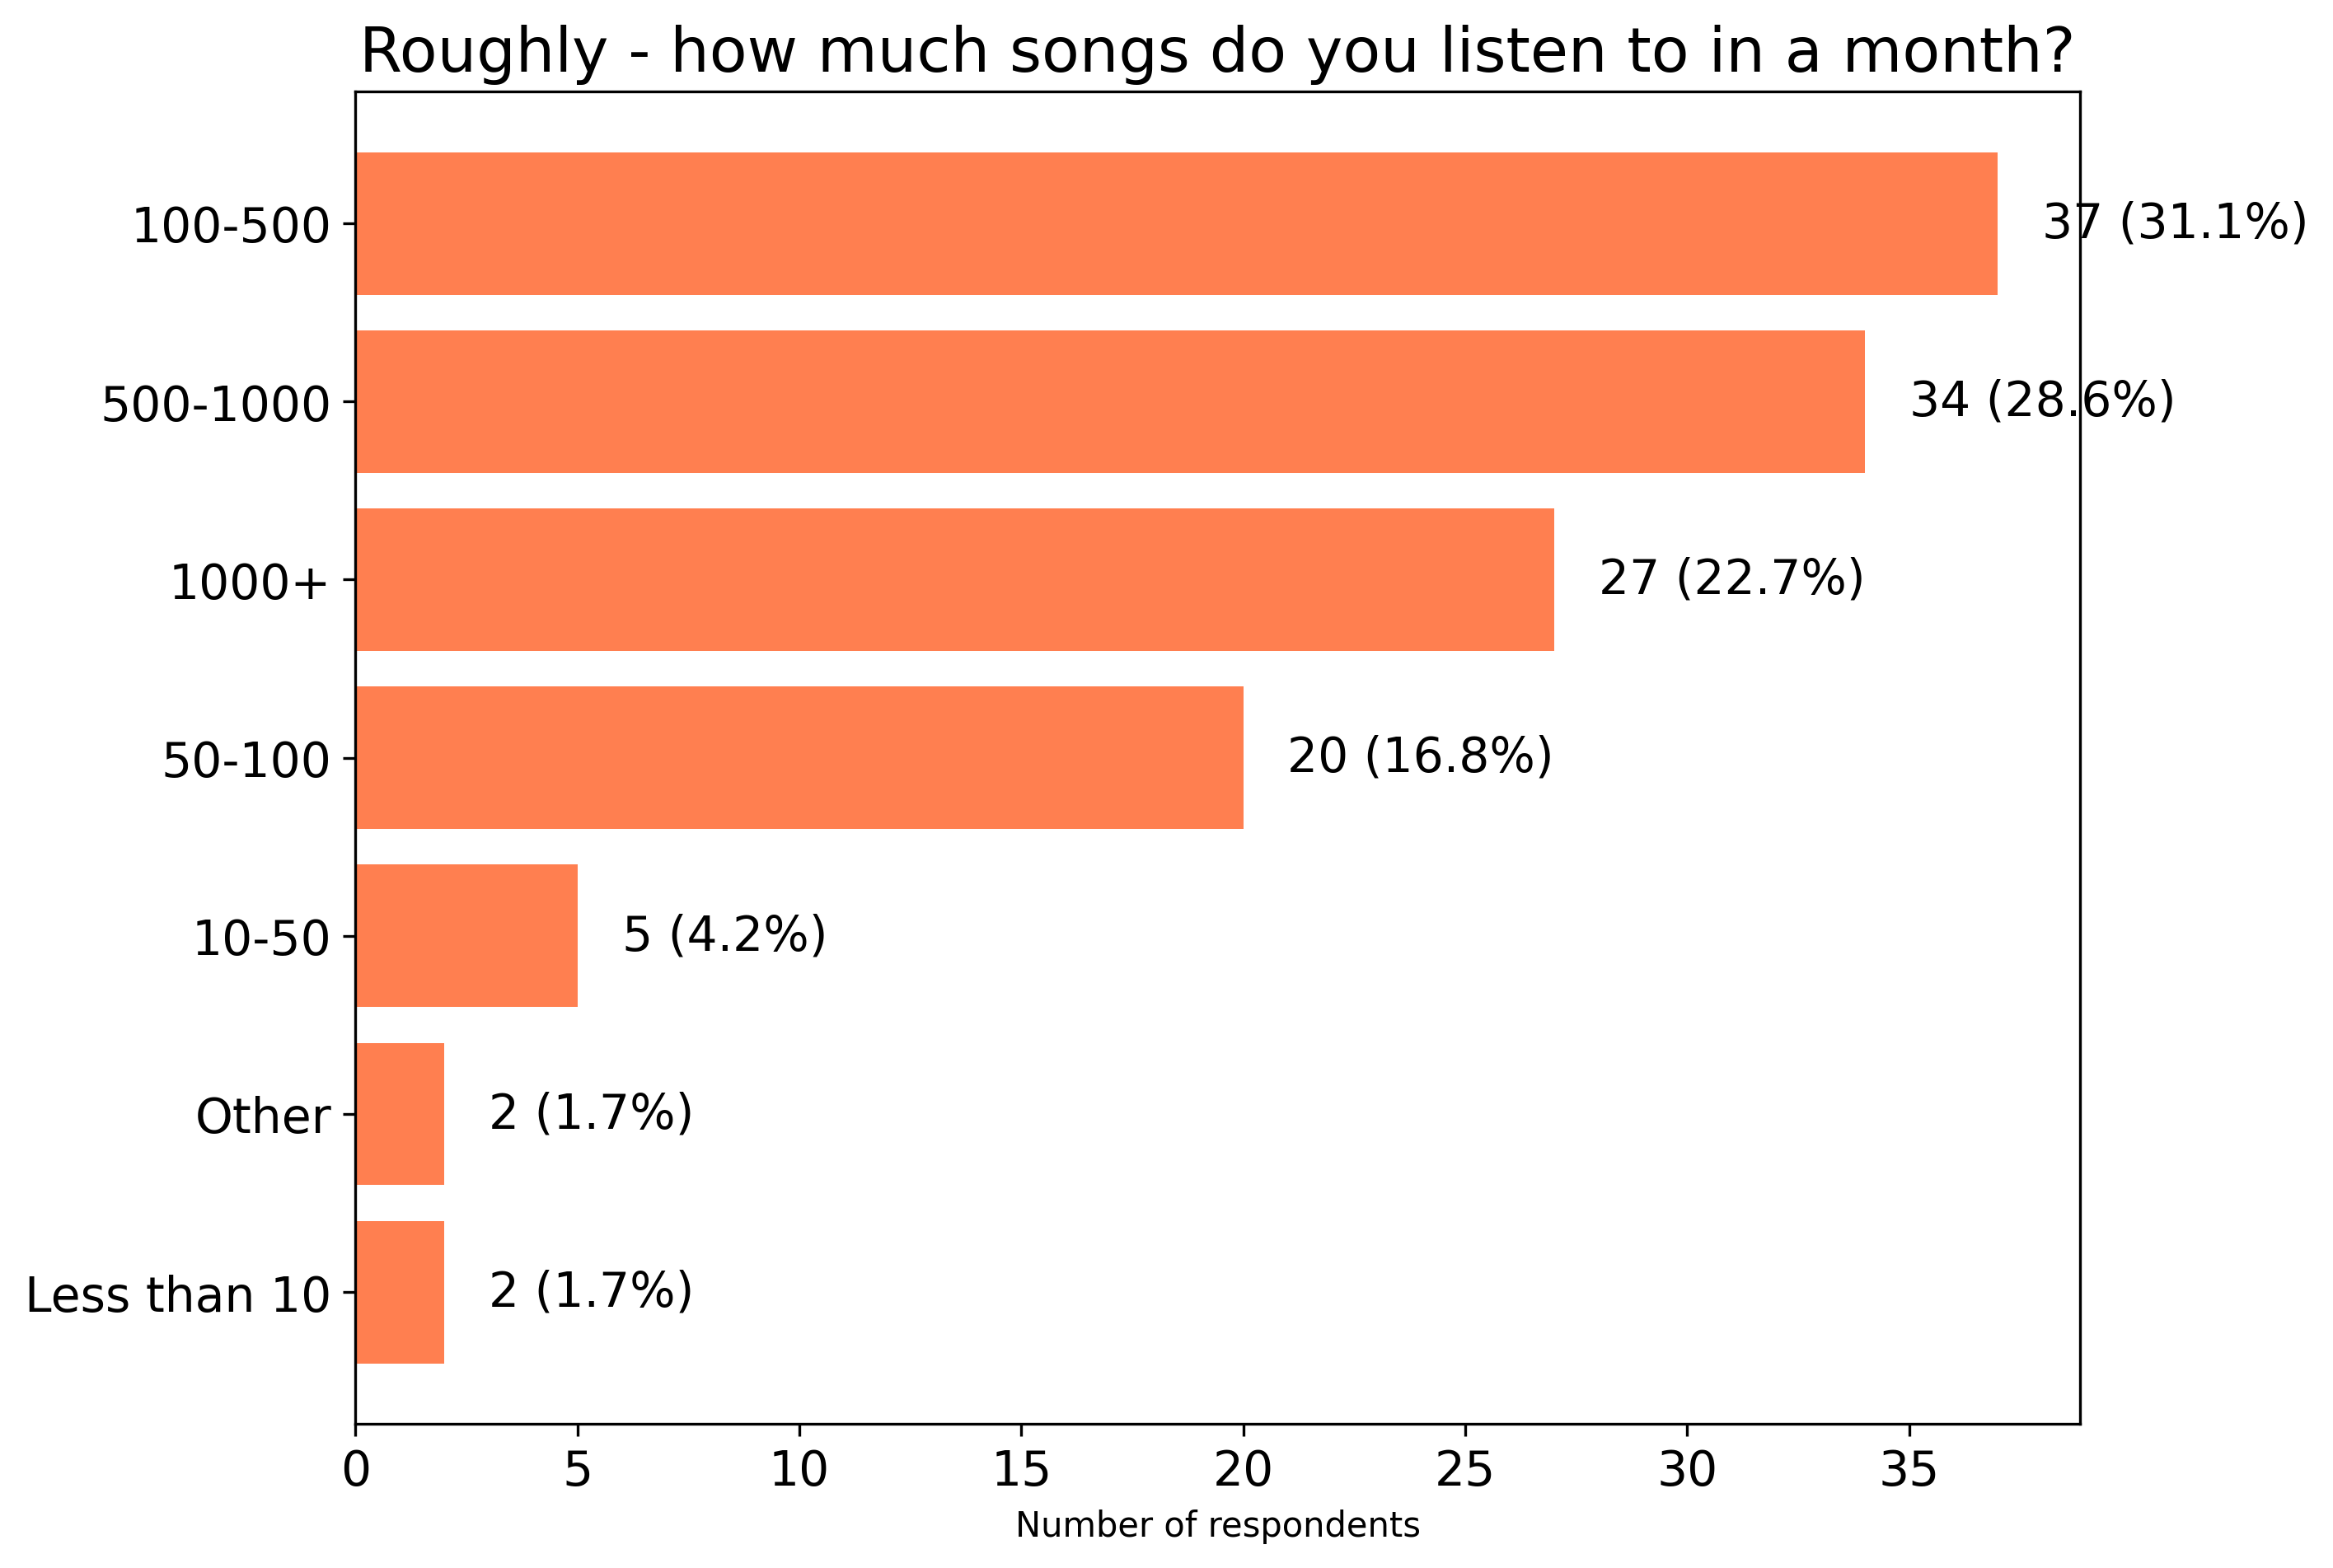
\includegraphics[height=0.4\textheight]{charts/song amount month.png}
    \caption{Monthly song count per respondent}
    \label{fig:song_amount}
\end{figure}

\begin{figure}[htbp]
    \centering
    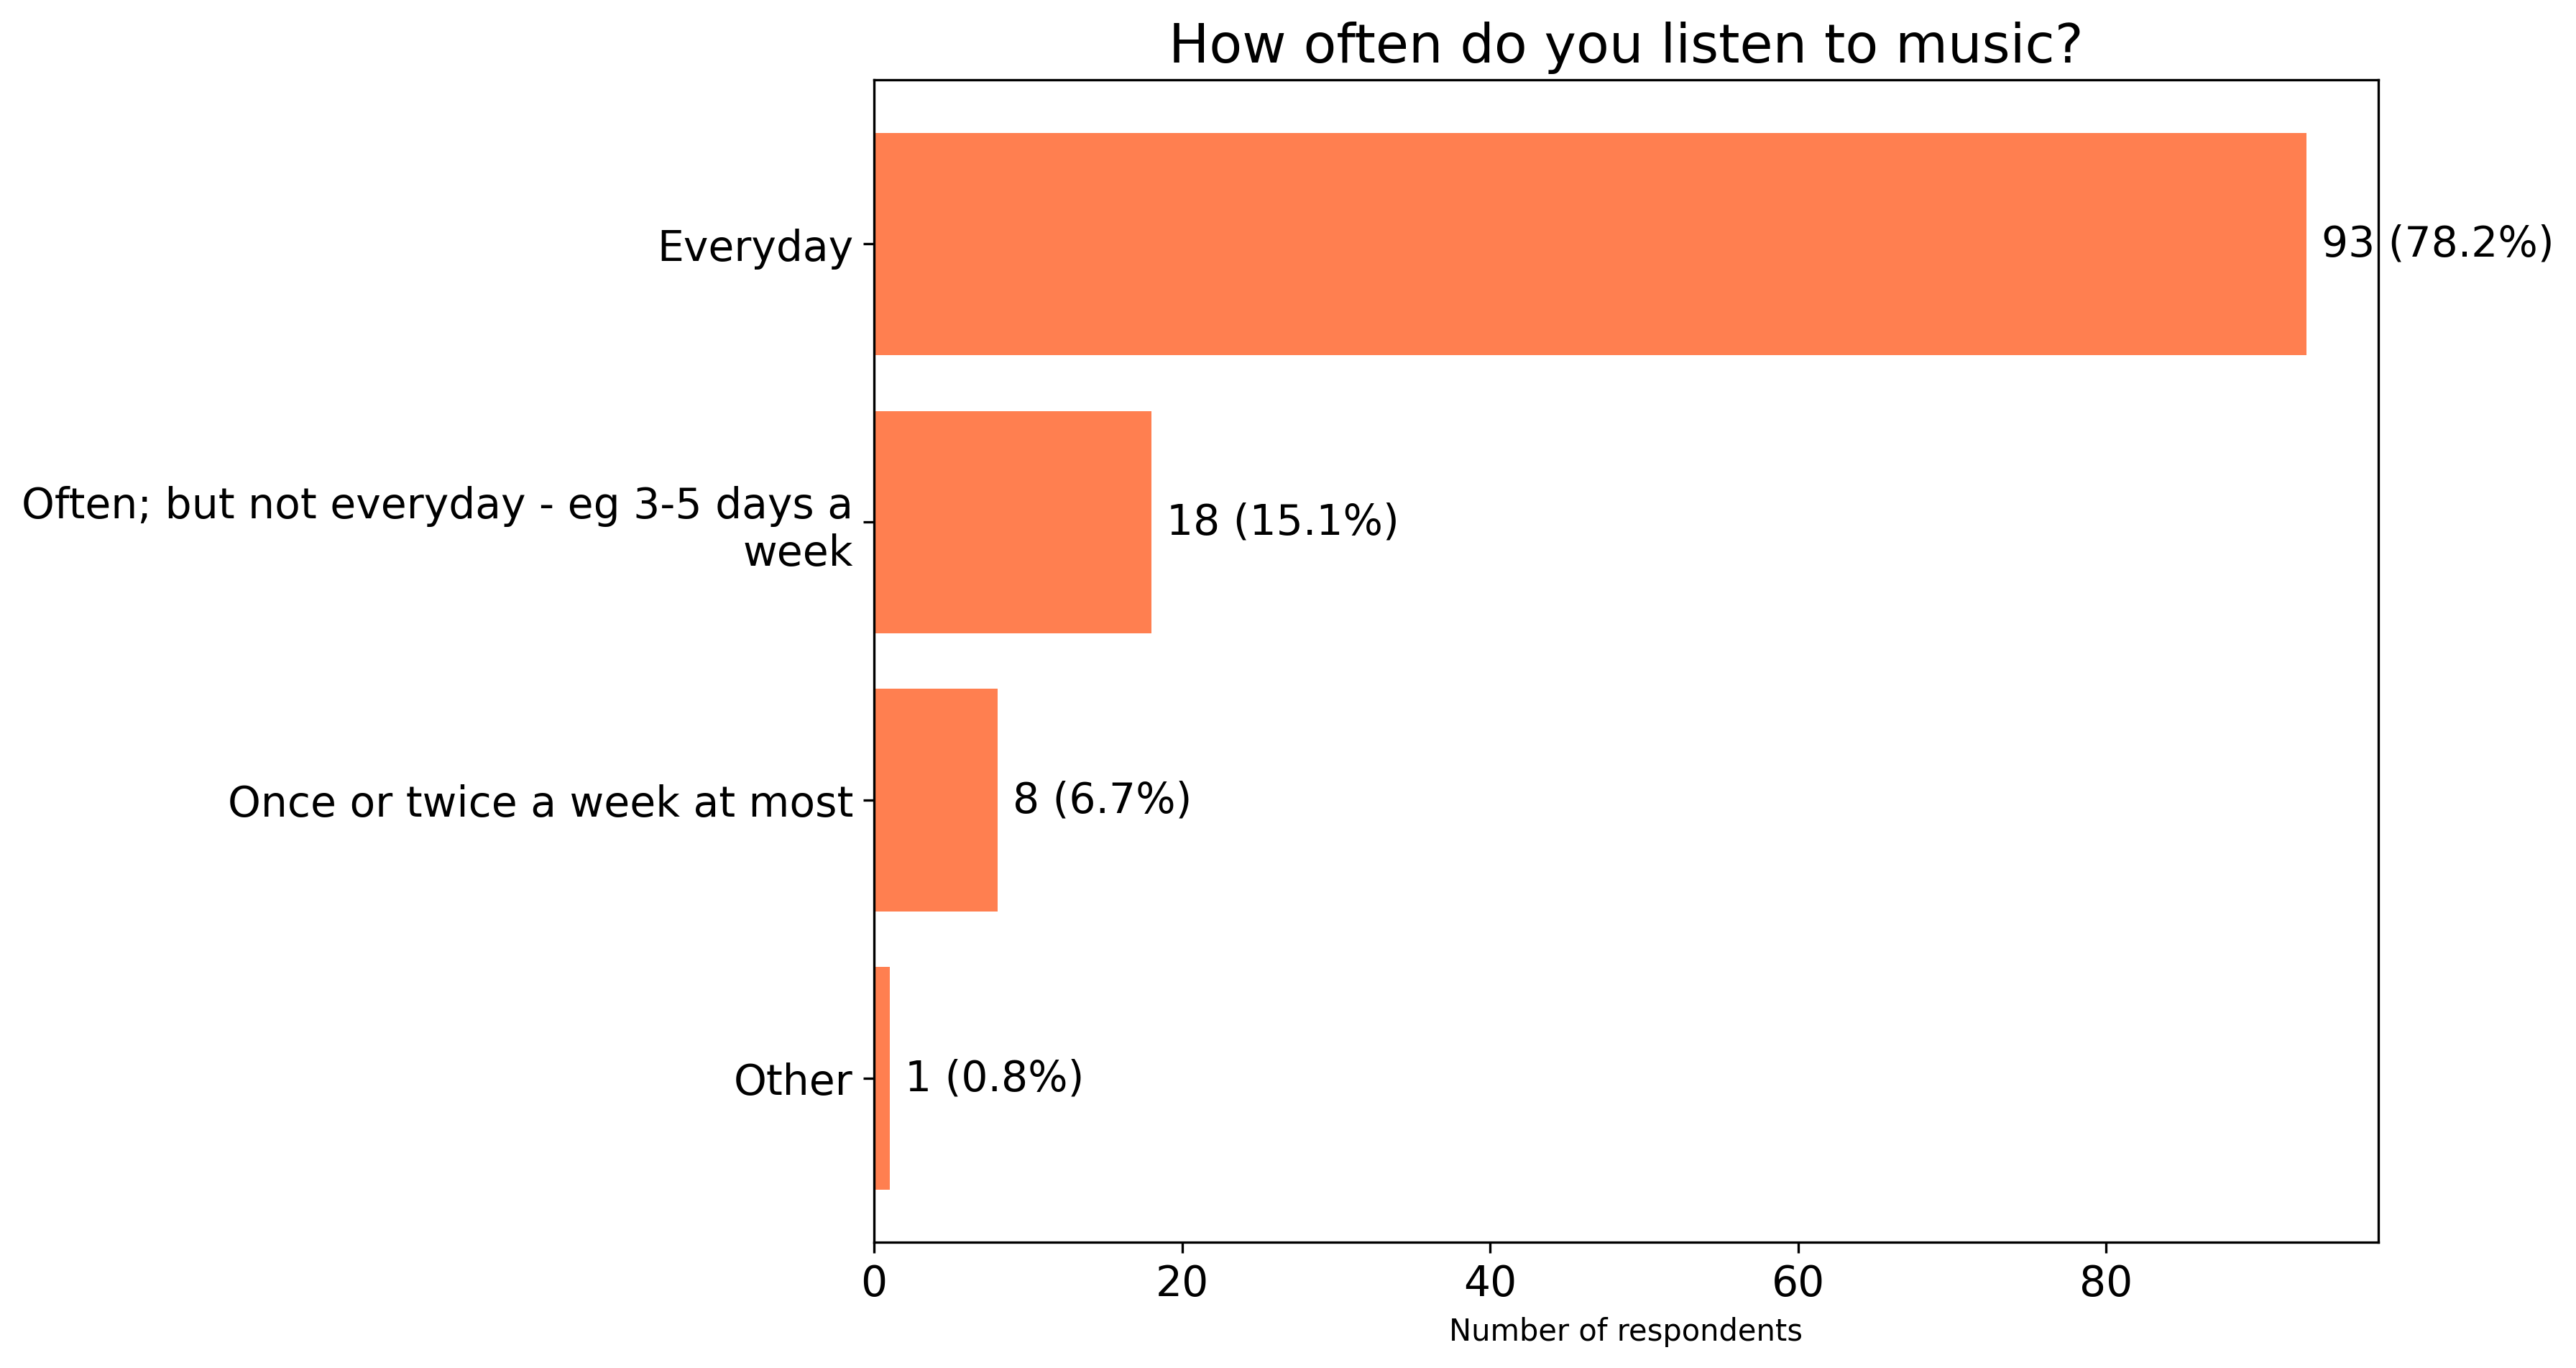
\includegraphics[height=0.4\textheight]{charts/listening regularity.png}
    \caption{Listening frequency of respondents}
    \label{fig:listen_reg}
\end{figure}

\subsection{Listening Methods}
As can be seen in Figure~\ref{fig:consumption_methods} the percentage of streaming platforms
usage across all ages is nearing 100\% with slightly higher numbers in lower age groups.
Although, downloaded files and physical media have their presence,
especially for people aged 30-60, it is usually only an auxiliary option next to the streaming solutions.

\begin{figure}[htbp]
    \centering
    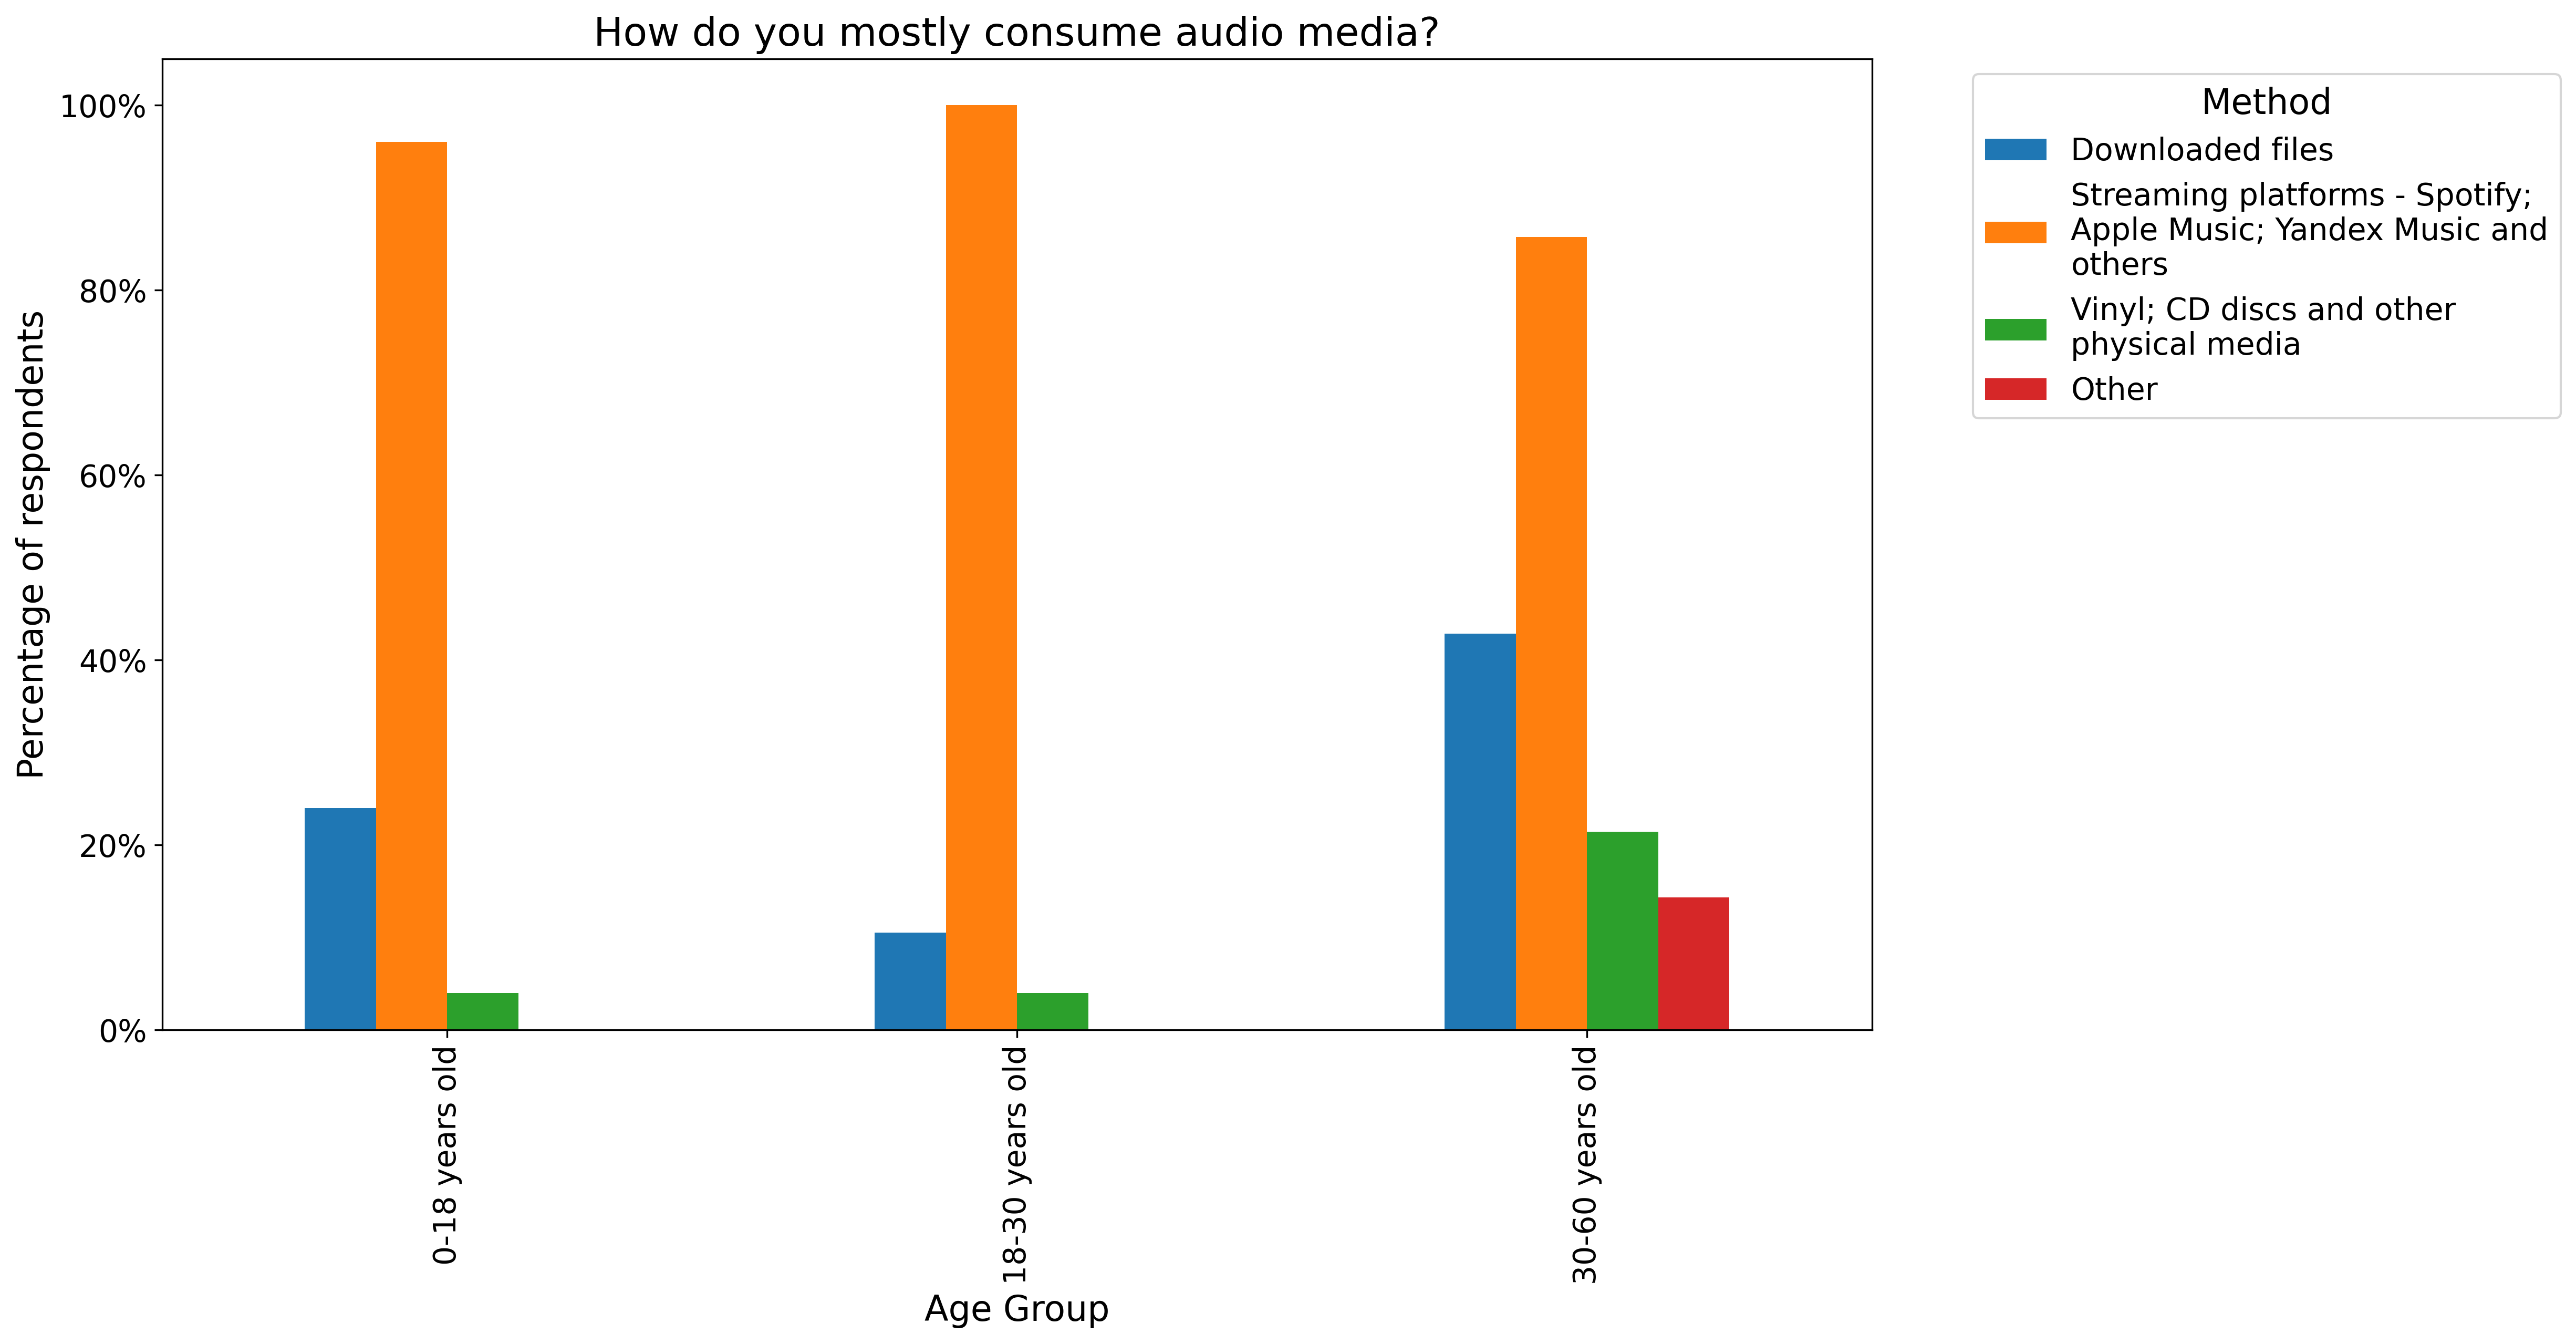
\includegraphics[height=0.4\textheight]{charts/constumption_method.png}
    \caption{Audio media consumption by age group}
    \label{fig:consumption_methods}
\end{figure}

Regarding the platforms themselves - Spotify has taken the first place in terms of popularity, proving the
global statistics\cite{spotifypopularity}. However, Yandex Music being in the second place deserves an explanation.
As mentioned previously, most of the respondents are from Russian-speaking countries, Russia specifically.
With a lot of western companies leaving its market in 2022, music streaming services included, most of the users has
moved to locally available products - Yandex Music, VK Music, Zvuk, and others.
Another notable point is the absence of other popular region-specific platforms, such as Amazon Music for the US market,
QQ music for the Chinese market or JioSaavn for the Indian one,
as all of the respondents were based in the european part of the world.
The full statistics are shown in Figure~\ref{fig:platform_popularity}.

\begin{figure}[htbp]
    \centering
    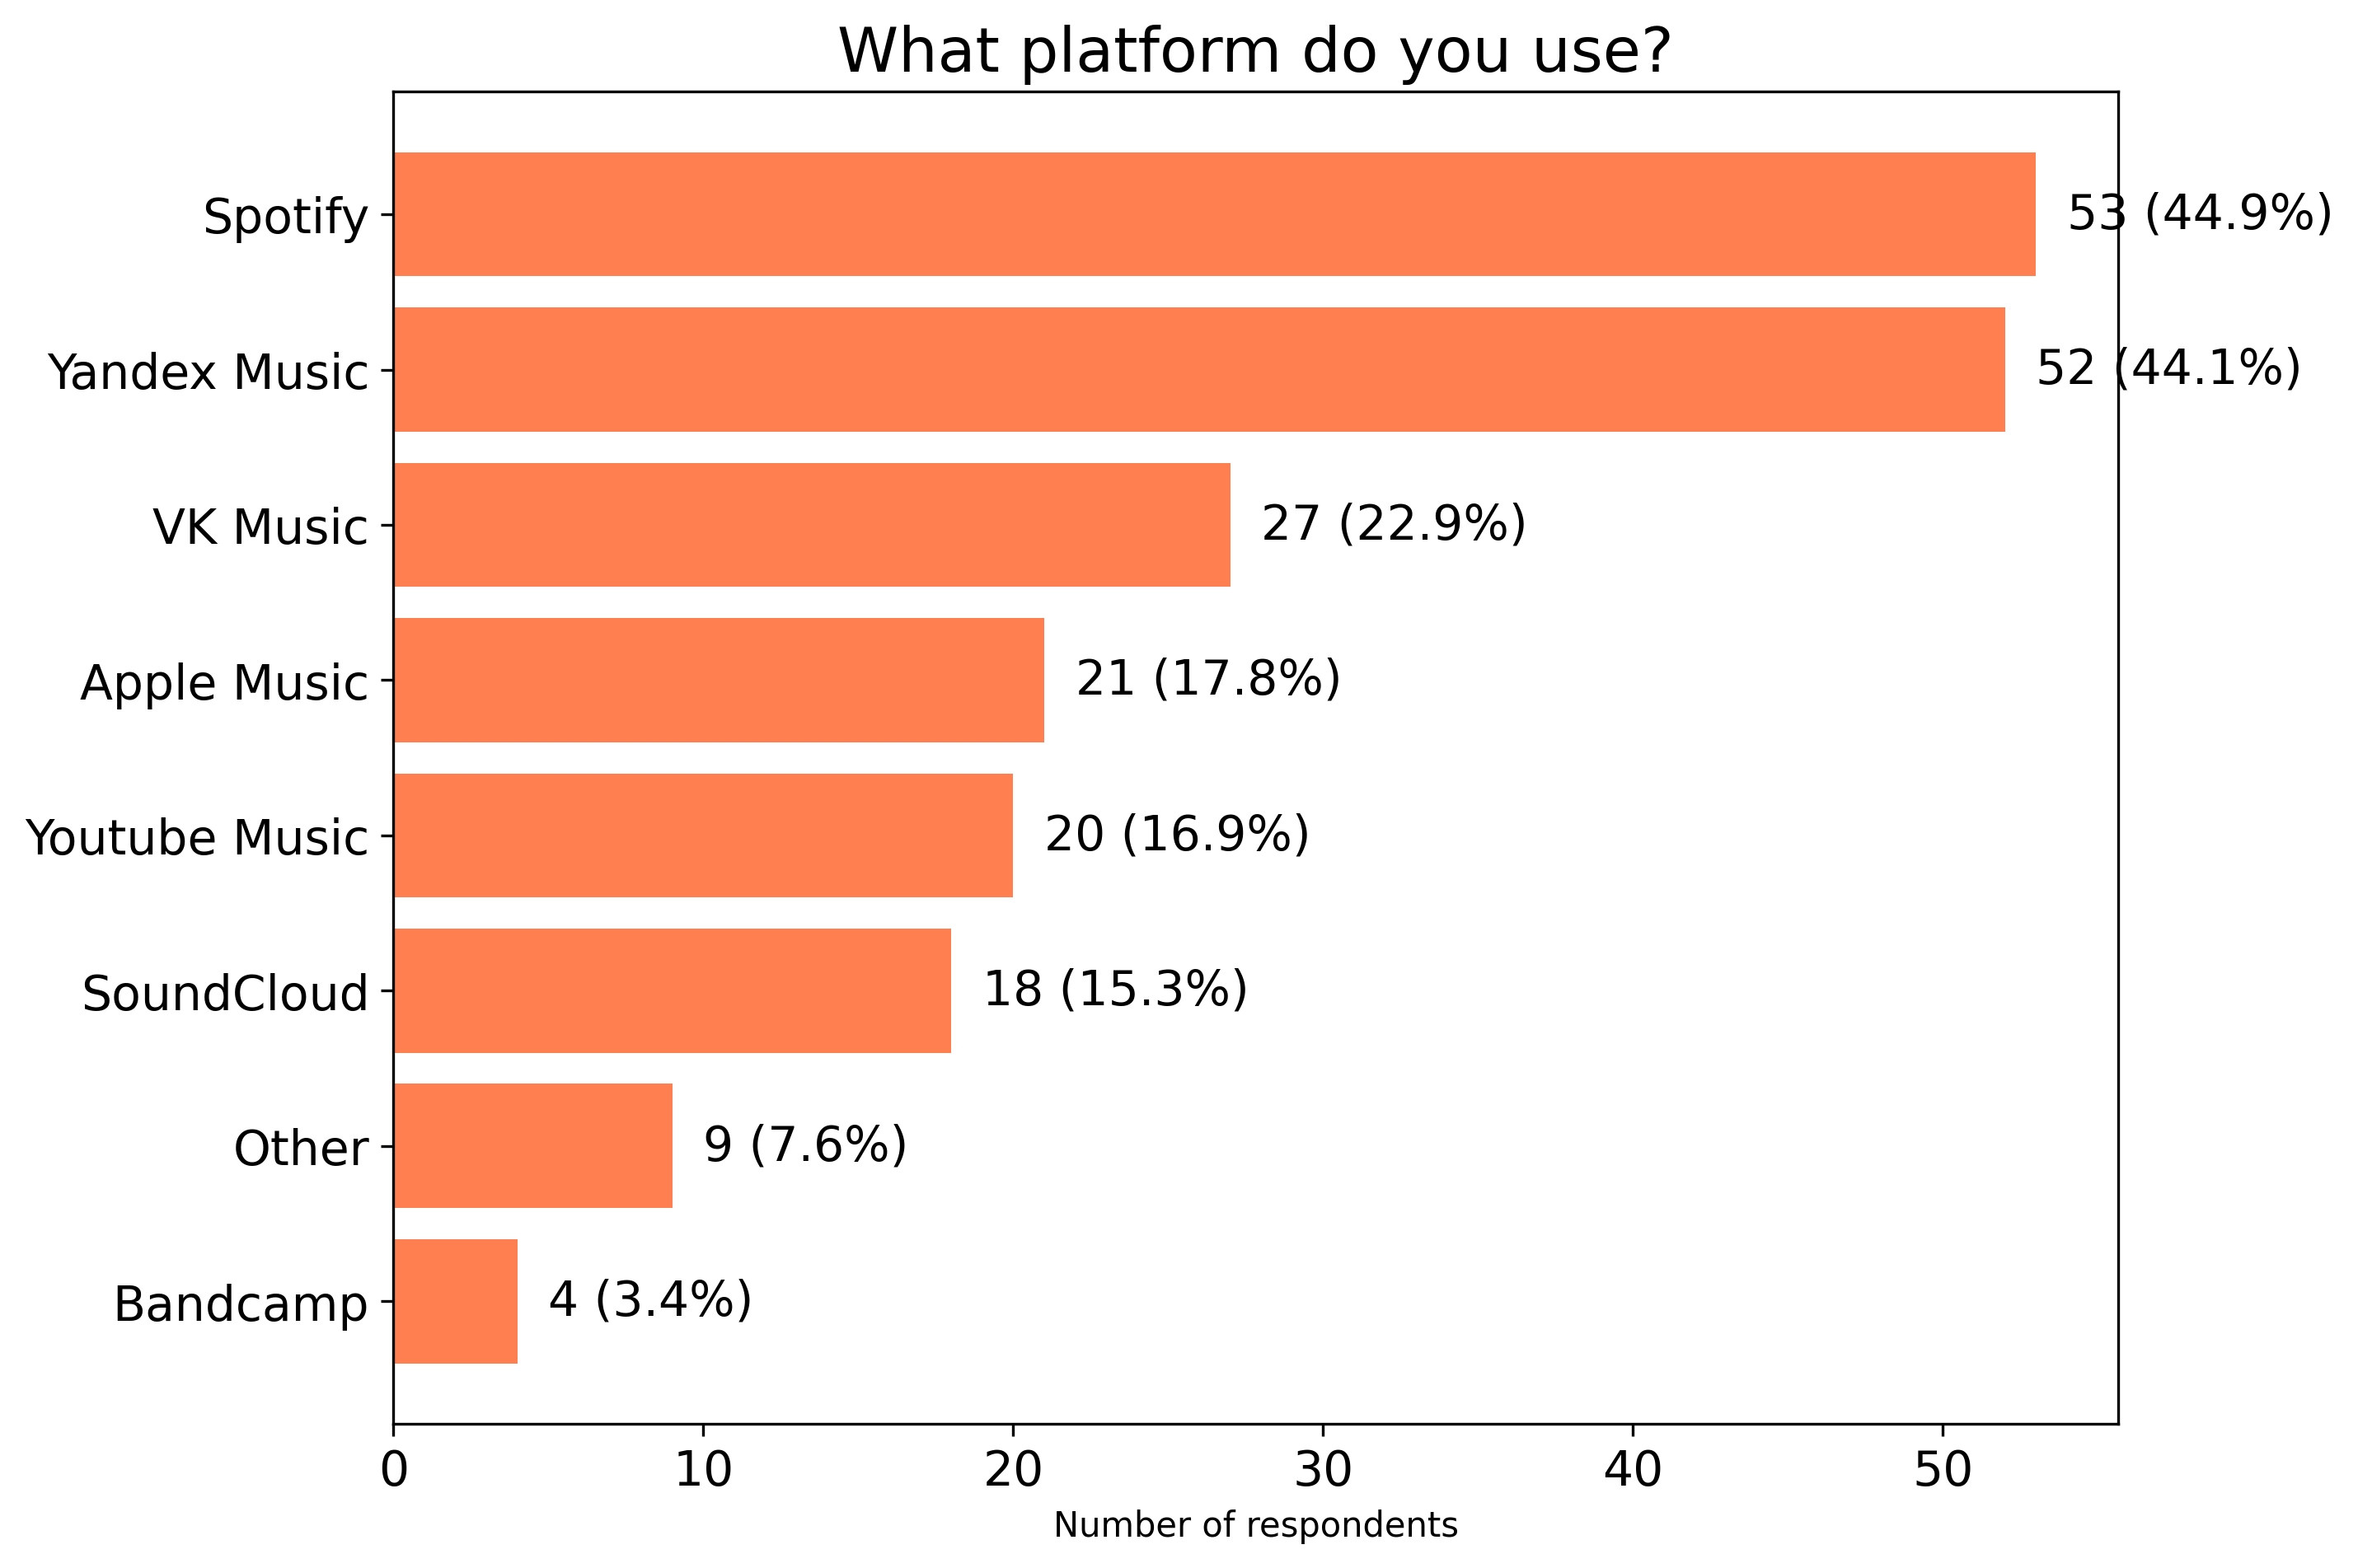
\includegraphics[height=0.4\textheight]{charts/streaming platform.png}
    \caption{Streaming platforms popularity}
    \label{fig:platform_popularity}
\end{figure}

Being established that streaming services are indeed widely-used and are in demand, the next important step would be
to analyze the regularity of music-centered social interactions.

\subsection{Social Interactions}
The results of Question 10 indicate that nearly all respondents (99.2\%) reported listening to music with
others, primarily in offline settings such as gatherings or car rides (Figure~\ref{fig:listentogethermeth}).
Online co-listening methods, while less common, were also mentioned by a quarter of respondents,
showing that digital solutions for shared listening are used, though not as prevalently as in-person scenarios.

\begin{figure}[htbp]
    \centering
    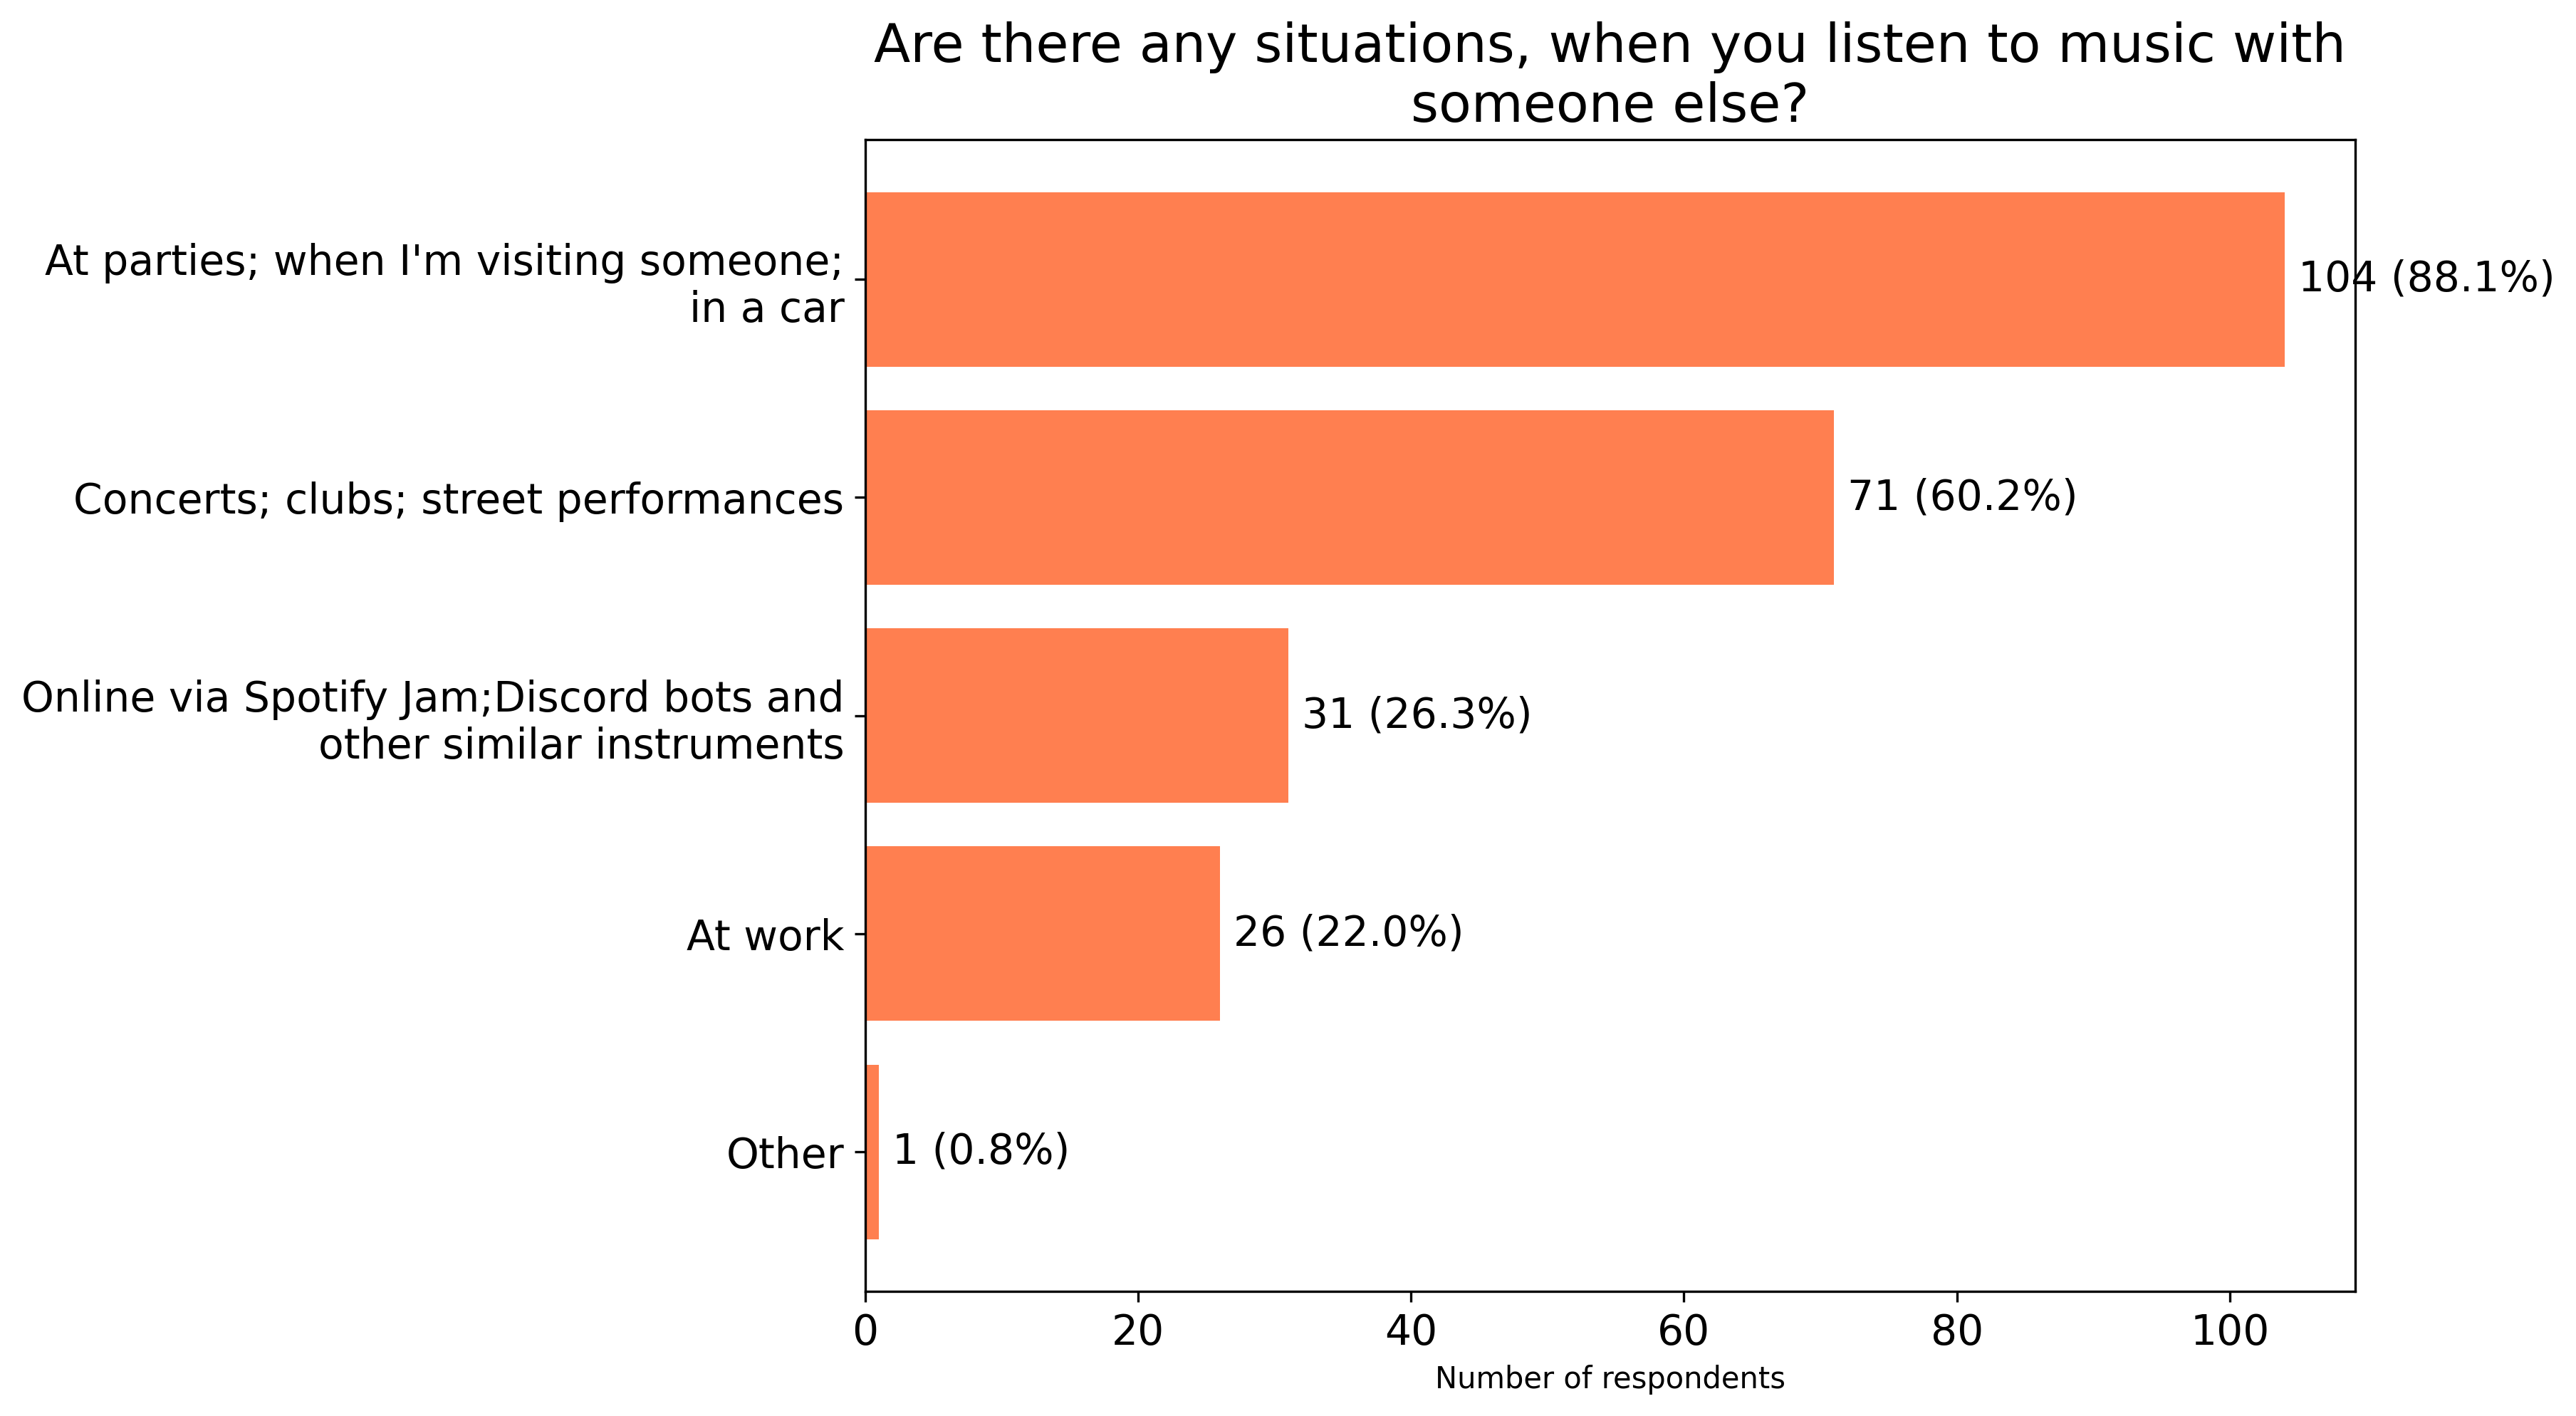
\includegraphics[height=0.4\textheight]{charts/listen together method.png}
    \caption{Social interaction methods}
    \label{fig:listentogethermeth}
\end{figure}

Question 11 (Figure~\ref{fig:listentogetherfreq}) investigates how often these interactions occur —
the results show that a significant portion of respondents engage in shared listening regularly.
Around 60\% reported doing so at least a few times per month,
with a smaller group indicating almost daily interactions.
This reinforces the idea that music consumption is a common social activity.


\begin{figure}[htbp]
    \centering
    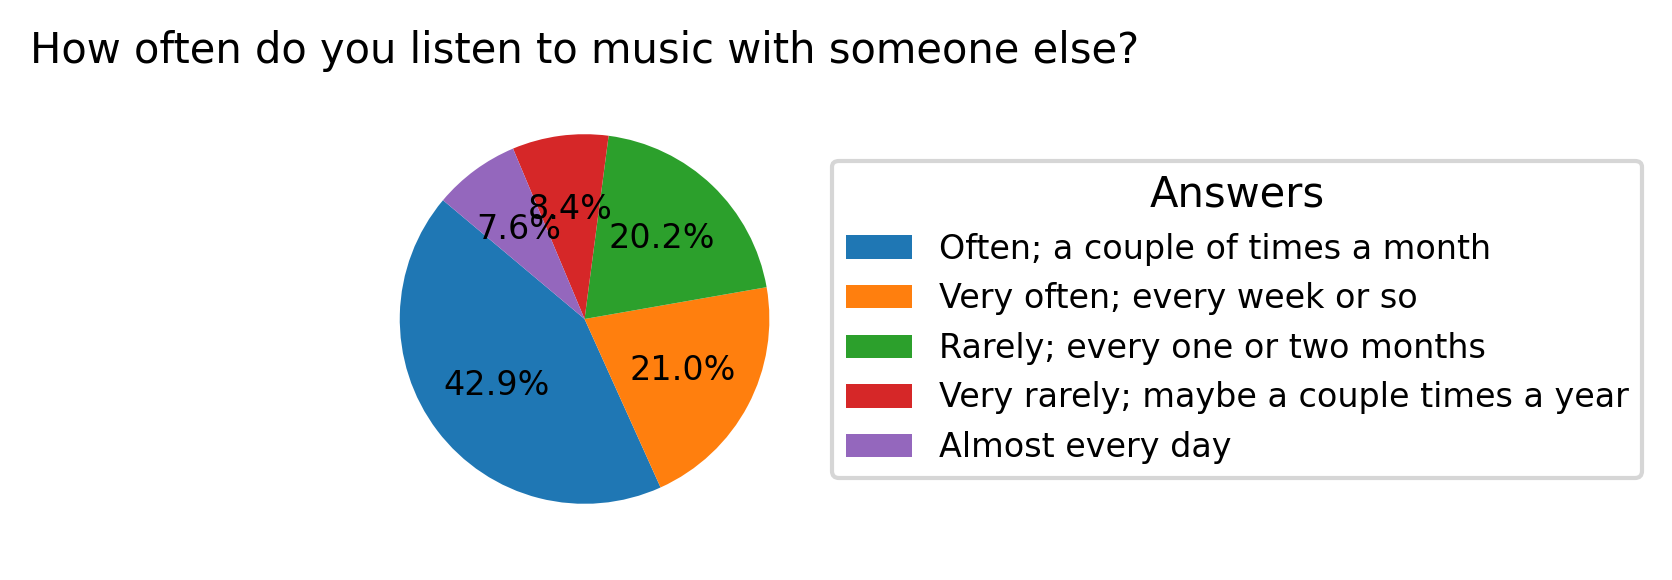
\includegraphics[width=1\textwidth, keepaspectratio]{charts/listen together freq.png}
    \caption{Social interactions frequency}
    \label{fig:listentogetherfreq}
\end{figure}

The next question is phrased as following - "How often do you/your friends share/discuss music?".
While the previous question focused on real-time in-person collective listening,
this one highlights more intentional and in-depth musical interactions — such as sharing songs,
recommending music, or discussing it. Music in that case is not just the background but the main subject of engagement.
The same trend as before can be observed in the responses: a majority of participants reported engaging in these exchanges regularly.
Over 70\% (Figure~\ref{fig:sharefreq}) indicated that they share music at least several times a month, with many doing so weekly or more often.
This further emphasizes the active social role of music.

\begin{figure}[htbp]
    \centering
    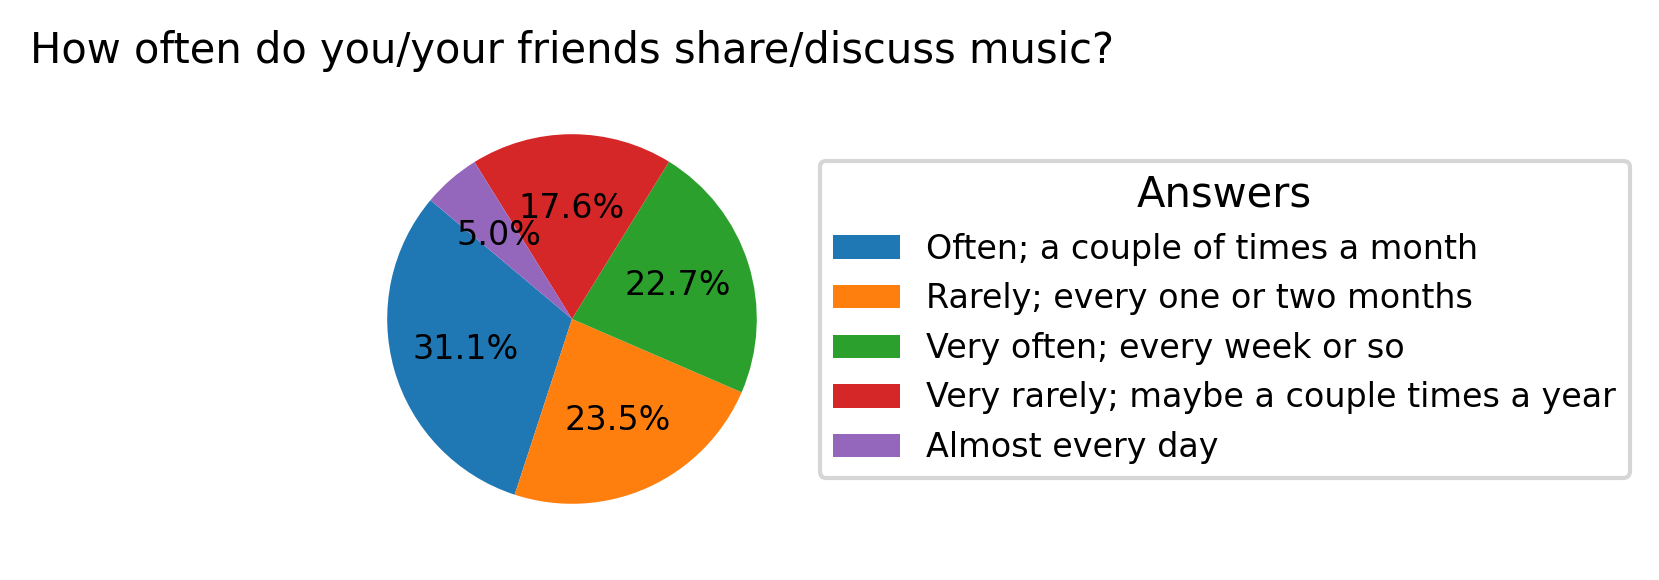
\includegraphics[width=1\textwidth, keepaspectratio]{charts/share freq.png}
    \caption{Music sharing frequency}
    \label{fig:sharefreq}
\end{figure}

Question 13 — “How does that happen?” (as in music sharing) — provides an insight into the specific means of sharing.
Many respondents (Figure~\ref{fig:sharemeth}) stated that they typically send links from streaming platforms through external messaging apps.
While this shows a clear demand for sharing music online, it also reveals a gap: these interactions are fragmented across platforms.
Hence, enabling such exchanges directly within the streaming app could offer a smoother, more uniform experience.

\begin{figure}[htbp]
    \centering
    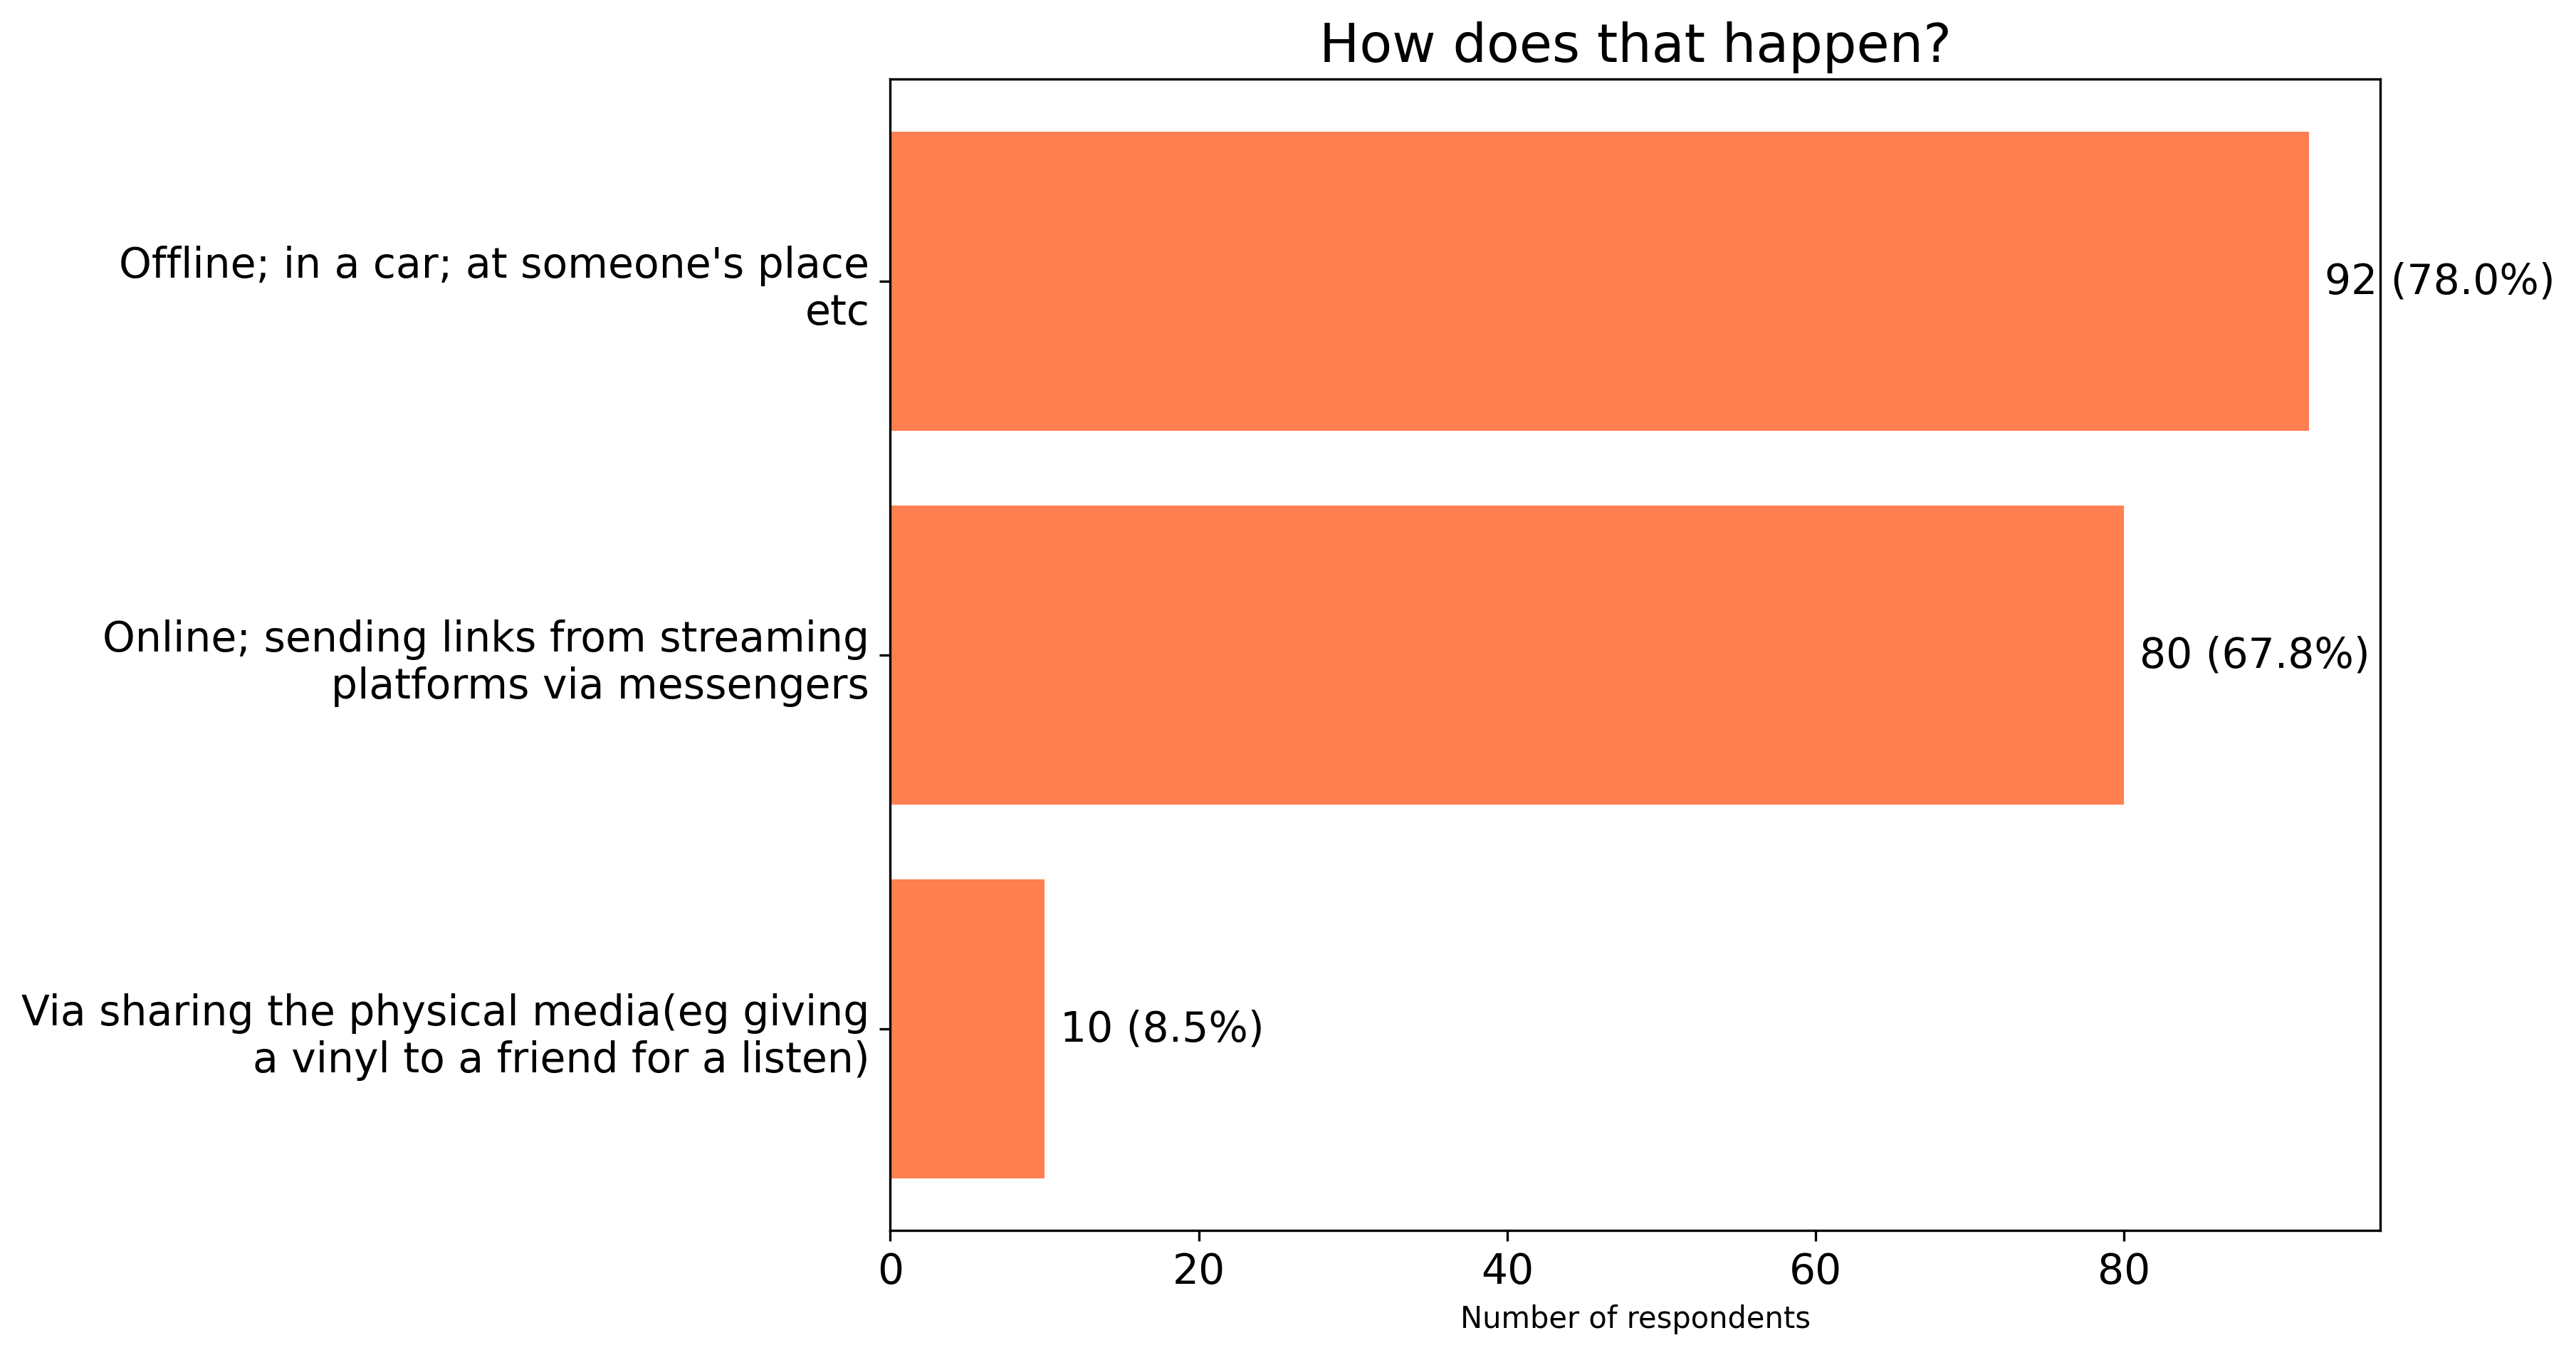
\includegraphics[height=0.4\textheight]{charts/share method.png}
    \caption{Music sharing methods}
    \label{fig:sharemeth}
\end{figure}

Responses to the question \textit{“Would you say that you know a lot of people with similar music taste?”} were mixed,
with a near-even split.
This suggests that while some users already have a social circle with similar music taste, many do not.
Interestingly, when asked
\textit{“Would you like to connect with others who share your musical taste, or influence those around you to explore and appreciate the music you enjoy?”},
the majority answered positively.
This indicates an interest in the expansion of musical connections and supports the idea that social discovery
features could be useful within a streaming platform.
This is further supported by the responses to Question 15, where over 60\% of participants stated they would use
additional social features, if available on a streaming platform.


\section{Summary}
Overall, the results show that music is a vital part of many peoples' lives
and that streaming services are the main way people listen to it.
It is easy to see that music consumption is frequent and often appears in social interactions.
Yet, current platforms only partly support the possibility for interactions with other users.
Therefore, the idea of a music streaming service with integrated social features could be relevant,
addressing real user needs.
